%% bare_jrnl.tex
%% V1.4b
%% 2015/08/26
%% by Michael Shell
%% see http://www.michaelshell.org/
%% for current contact information.
%%
%% This is a skeleton file demonstrating the use of IEEEtran.cls
%% (requires IEEEtran.cls version 1.8b or later) with an IEEE
%% journal paper.
%%
%% Support sites:
%% http://www.michaelshell.org/tex/ieeetran/
%% http://www.ctan.org/pkg/ieeetran
%% and
%% http://www.ieee.org/

%%*************************************************************************
%% Legal Notice:
%% This code is offered as-is without any warranty either expressed or
%% implied; without even the implied warranty of MERCHANTABILITY or
%% FITNESS FOR A PARTICULAR PURPOSE! 
%% User assumes all risk.
%% In no event shall the IEEE or any contributor to this code be liable for
%% any damages or losses, including, but not limited to, incidental,
%% consequential, or any other damages, resulting from the use or misuse
%% of any information contained here.
%%
%% All comments are the opinions of their respective authors and are not
%% necessarily endorsed by the IEEE.
%%
%% This work is distributed under the LaTeX Project Public License (LPPL)
%% ( http://www.latex-project.org/ ) version 1.3, and may be freely used,
%% distributed and modified. A copy of the LPPL, version 1.3, is included
%% in the base LaTeX documentation of all distributions of LaTeX released
%% 2003/12/01 or later.
%% Retain all contribution notices and credits.
%% ** Modified files should be clearly indicated as such, including  **
%% ** renaming them and changing author support contact information. **
%%*************************************************************************


% *** Authors should verify (and, if needed, correct) their LaTeX system  ***
% *** with the testflow diagnostic prior to trusting their LaTeX platform ***
% *** with production work. The IEEE's font choices and paper sizes can   ***
% *** trigger bugs that do not appear when using other class files.       ***                          ***
% The testflow support page is at:
% http://www.michaelshell.org/tex/testflow/



\documentclass[journal]{IEEEtran}
%
% If IEEEtran.cls has not been installed into the LaTeX system files,
% manually specify the path to it like:
% \documentclass[journal]{../sty/IEEEtran}





% Some very useful LaTeX packages include:
% (uncomment the ones you want to load)


% *** MISC UTILITY PACKAGES ***
%
%\usepackage{ifpdf}
% Heiko Oberdiek's ifpdf.sty is very useful if you need conditional
% compilation based on whether the output is pdf or dvi.
% usage:
% \ifpdf
%   % pdf code
% \else
%   % dvi code
% \fi
% The latest version of ifpdf.sty can be obtained from:
% http://www.ctan.org/pkg/ifpdf
% Also, note that IEEEtran.cls V1.7 and later provides a builtin
% \ifCLASSINFOpdf conditional that works the same way.
% When switching from latex to pdflatex and vice-versa, the compiler may
% have to be run twice to clear warning/error messages.






% *** CITATION PACKAGES ***
%
%\usepackage{cite}
% cite.sty was written by Donald Arseneau
% V1.6 and later of IEEEtran pre-defines the format of the cite.sty package
% \cite{} output to follow that of the IEEE. Loading the cite package will
% result in citation numbers being automatically sorted and properly
% "compressed/ranged". e.g., [1], [9], [2], [7], [5], [6] without using
% cite.sty will become [1], [2], [5]--[7], [9] using cite.sty. cite.sty's
% \cite will automatically add leading space, if needed. Use cite.sty's
% noadjust option (cite.sty V3.8 and later) if you want to turn this off
% such as if a citation ever needs to be enclosed in parenthesis.
% cite.sty is already installed on most LaTeX systems. Be sure and use
% version 5.0 (2009-03-20) and later if using hyperref.sty.
% The latest version can be obtained at:
% http://www.ctan.org/pkg/cite
% The documentation is contained in the cite.sty file itself.






% *** GRAPHICS RELATED PACKAGES ***
\usepackage[pdftex]{graphicx}
%
\ifCLASSINFOpdf
  % \usepackage[pdftex]{graphicx}
  % declare the path(s) where your graphic files are
  % \graphicspath{{../pdf/}{../jpeg/}}
  % and their extensions so you won't have to specify these with
  % every instance of \includegraphics
  % \DeclareGraphicsExtensions{.pdf,.jpeg,.png}
\else
  % or other class option (dvipsone, dvipdf, if not using dvips). graphicx
  % will default to the driver specified in the system graphics.cfg if no
  % driver is specified.
   \usepackage[dvips]{graphicx}
  % declare the path(s) where your graphic files are
  % \graphicspath{{../eps/}}
  % and their extensions so you won't have to specify these with
  % every instance of \includegraphics
  % \DeclareGraphicsExtensions{.eps}
\fi
% graphicx was written by David Carlisle and Sebastian Rahtz. It is
% required if you want graphics, photos, etc. graphicx.sty is already
% installed on most LaTeX systems. The latest version and documentation
% can be obtained at: 
% http://www.ctan.org/pkg/graphicx
% Another good source of documentation is "Using Imported Graphics in
% LaTeX2e" by Keith Reckdahl which can be found at:
% http://www.ctan.org/pkg/epslatex
%
% latex, and pdflatex in dvi mode, support graphics in encapsulated
% postscript (.eps) format. pdflatex in pdf mode supports graphics
% in .pdf, .jpeg, .png and .mps (metapost) formats. Users should ensure
% that all non-photo figures use a vector format (.eps, .pdf, .mps) and
% not a bitmapped formats (.jpeg, .png). The IEEE frowns on bitmapped formats
% which can result in "jaggedy"/blurry rendering of lines and letters as
% well as large increases in file sizes.
%
% You can find documentation about the pdfTeX application at:
% http://www.tug.org/applications/pdftex





% *** MATH PACKAGES ***
%
%\usepackage{amsmath}
% A popular package from the American Mathematical Society that provides
% many useful and powerful commands for dealing with mathematics.
%
% Note that the amsmath package sets \interdisplaylinepenalty to 10000
% thus preventing page breaks from occurring within multiline equations. Use:
%\interdisplaylinepenalty=2500
% after loading amsmath to restore such page breaks as IEEEtran.cls normally
% does. amsmath.sty is already installed on most LaTeX systems. The latest
% version and documentation can be obtained at:
% http://www.ctan.org/pkg/amsmath





% *** SPECIALIZED LIST PACKAGES ***
%
%\usepackage{algorithmic}
% algorithmic.sty was written by Peter Williams and Rogerio Brito.
% This package provides an algorithmic environment fo describing algorithms.
% You can use the algorithmic environment in-text or within a figure
% environment to provide for a floating algorithm. Do NOT use the algorithm
% floating environment provided by algorithm.sty (by the same authors) or
% algorithm2e.sty (by Christophe Fiorio) as the IEEE does not use dedicated
% algorithm float types and packages that provide these will not provide
% correct IEEE style captions. The latest version and documentation of
% algorithmic.sty can be obtained at:
% http://www.ctan.org/pkg/algorithms
% Also of interest may be the (relatively newer and more customizable)
% algorithmicx.sty package by Szasz Janos:
% http://www.ctan.org/pkg/algorithmicx




% *** ALIGNMENT PACKAGES ***
%
%\usepackage{array}
% Frank Mittelbach's and David Carlisle's array.sty patches and improves
% the standard LaTeX2e array and tabular environments to provide better
% appearance and additional user controls. As the default LaTeX2e table
% generation code is lacking to the point of almost being broken with
% respect to the quality of the end results, all users are strongly
% advised to use an enhanced (at the very least that provided by array.sty)
% set of table tools. array.sty is already installed on most systems. The
% latest version and documentation can be obtained at:
% http://www.ctan.org/pkg/array


% IEEEtran contains the IEEEeqnarray family of commands that can be used to
% generate multiline equations as well as matrices, tables, etc., of high
% quality.




% *** SUBFIGURE PACKAGES ***
%\ifCLASSOPTIONcompsoc
%  \usepackage[caption=false,font=normalsize,labelfont=sf,textfont=sf]{subfig}
%\else
%  \usepackage[caption=false,font=footnotesize]{subfig}
%\fi
% subfig.sty, written by Steven Douglas Cochran, is the modern replacement
% for subfigure.sty, the latter of which is no longer maintained and is
% incompatible with some LaTeX packages including fixltx2e. However,
% subfig.sty requires and automatically loads Axel Sommerfeldt's caption.sty
% which will override IEEEtran.cls' handling of captions and this will result
% in non-IEEE style figure/table captions. To prevent this problem, be sure
% and invoke subfig.sty's "caption=false" package option (available since
% subfig.sty version 1.3, 2005/06/28) as this is will preserve IEEEtran.cls
% handling of captions.
% Note that the Computer Society format requires a larger sans serif font
% than the serif footnote size font used in traditional IEEE formatting
% and thus the need to invoke different subfig.sty package options depending
% on whether compsoc mode has been enabled.
%
% The latest version and documentation of subfig.sty can be obtained at:
% http://www.ctan.org/pkg/subfig




% *** FLOAT PACKAGES ***
%
%\usepackage{fixltx2e}
% fixltx2e, the successor to the earlier fix2col.sty, was written by
% Frank Mittelbach and David Carlisle. This package corrects a few problems
% in the LaTeX2e kernel, the most notable of which is that in current
% LaTeX2e releases, the ordering of single and double column floats is not
% guaranteed to be preserved. Thus, an unpatched LaTeX2e can allow a
% single column figure to be placed prior to an earlier double column
% figure.
% Be aware that LaTeX2e kernels dated 2015 and later have fixltx2e.sty's
% corrections already built into the system in which case a warning will
% be issued if an attempt is made to load fixltx2e.sty as it is no longer
% needed.
% The latest version and documentation can be found at:
% http://www.ctan.org/pkg/fixltx2e


%\usepackage{stfloats}
% stfloats.sty was written by Sigitas Tolusis. This package gives LaTeX2e
% the ability to do double column floats at the bottom of the page as well
% as the top. (e.g., "\begin{figure*}[!b]" is not normally possible in
% LaTeX2e). It also provides a command:
%\fnbelowfloat
% to enable the placement of footnotes below bottom floats (the standard
% LaTeX2e kernel puts them above bottom floats). This is an invasive package
% which rewrites many portions of the LaTeX2e float routines. It may not work
% with other packages that modify the LaTeX2e float routines. The latest
% version and documentation can be obtained at:
% http://www.ctan.org/pkg/stfloats
% Do not use the stfloats baselinefloat ability as the IEEE does not allow
% \baselineskip to stretch. Authors submitting work to the IEEE should note
% that the IEEE rarely uses double column equations and that authors should try
% to avoid such use. Do not be tempted to use the cuted.sty or midfloat.sty
% packages (also by Sigitas Tolusis) as the IEEE does not format its papers in
% such ways.
% Do not attempt to use stfloats with fixltx2e as they are incompatible.
% Instead, use Morten Hogholm'a dblfloatfix which combines the features
% of both fixltx2e and stfloats:
%
% \usepackage{dblfloatfix}
% The latest version can be found at:
% http://www.ctan.org/pkg/dblfloatfix




%\ifCLASSOPTIONcaptionsoff
%  \usepackage[nomarkers]{endfloat}
% \let\MYoriglatexcaption\caption
% \renewcommand{\caption}[2][\relax]{\MYoriglatexcaption[#2]{#2}}
%\fi
% endfloat.sty was written by James Darrell McCauley, Jeff Goldberg and 
% Axel Sommerfeldt. This package may be useful when used in conjunction with 
% IEEEtran.cls'  captionsoff option. Some IEEE journals/societies require that
% submissions have lists of figures/tables at the end of the paper and that
% figures/tables without any captions are placed on a page by themselves at
% the end of the document. If needed, the draftcls IEEEtran class option or
% \CLASSINPUTbaselinestretch interface can be used to increase the line
% spacing as well. Be sure and use the nomarkers option of endfloat to
% prevent endfloat from "marking" where the figures would have been placed
% in the text. The two hack lines of code above are a slight modification of
% that suggested by in the endfloat docs (section 8.4.1) to ensure that
% the full captions always appear in the list of figures/tables - even if
% the user used the short optional argument of \caption[]{}.
% IEEE papers do not typically make use of \caption[]'s optional argument,
% so this should not be an issue. A similar trick can be used to disable
% captions of packages such as subfig.sty that lack options to turn off
% the subcaptions:
% For subfig.sty:
% \let\MYorigsubfloat\subfloat
% \renewcommand{\subfloat}[2][\relax]{\MYorigsubfloat[]{#2}}
% However, the above trick will not work if both optional arguments of
% the \subfloat command are used. Furthermore, there needs to be a
% description of each subfigure *somewhere* and endfloat does not add
% subfigure captions to its list of figures. Thus, the best approach is to
% avoid the use of subfigure captions (many IEEE journals avoid them anyway)
% and instead reference/explain all the subfigures within the main caption.
% The latest version of endfloat.sty and its documentation can obtained at:
% http://www.ctan.org/pkg/endfloat
%
% The IEEEtran \ifCLASSOPTIONcaptionsoff conditional can also be used
% later in the document, say, to conditionally put the References on a 
% page by themselves.




% *** PDF, URL AND HYPERLINK PACKAGES ***
%
%\usepackage{url}
% url.sty was written by Donald Arseneau. It provides better support for
% handling and breaking URLs. url.sty is already installed on most LaTeX
% systems. The latest version and documentation can be obtained at:
% http://www.ctan.org/pkg/url
% Basically, \url{my_url_here}.




% *** Do not adjust lengths that control margins, column widths, etc. ***
% *** Do not use packages that alter fonts (such as pslatex).         ***
% There should be no need to do such things with IEEEtran.cls V1.6 and later.
% (Unless specifically asked to do so by the journal or conference you plan
% to submit to, of course. )


% correct bad hyphenation here
\hyphenation{op-tical net-works semi-conduc-tor}


\begin{document}
%
% paper title
% Titles are generally capitalized except for words such as a, an, and, as,
% at, but, by, for, in, nor, of, on, or, the, to and up, which are usually
% not capitalized unless they are the first or last word of the title.
% Linebreaks \\ can be used within to get better formatting as desired.
% Do not put math or special symbols in the title.
\title{Wearable Medical Devices: A Comprehensive Review of Applications, Materials, and Future Directions}
%
%
% author names and IEEE memberships
% note positions of commas and nonbreaking spaces ( ~ ) LaTeX will not break
% a structure at a ~ so this keeps an author's name from being broken across
% two lines.
% use \thanks{} to gain access to the first footnote area
% a separate \thanks must be used for each paragraph as LaTeX2e's \thanks
% was not built to handle multiple paragraphs
%

\author{Ana~Camarinha,
        Daniel~Proaño-Guevara,
        Evangelia~Antoniadi,
        Miguel~Campos% <-this % stops a space

\thanks{All authors contributed equally for this work. Their names appear in alphabetical order.}% <-this % stops a space
\thanks{This research paper has utilized language models, including ChatGPT and Writefull, for assistance in language correction, editing, and enhancing clarity during the redaction process. Although these tools were used to support the authors in achieving high technical and linguistic standards, the authors retain full responsibility for the accuracy, validity, and originality of the content presented herein. The use of AI-based tools does not diminish the authors’ accountability for the integrity and authenticity of the work.}% <-this % stops a space
\thanks{Manuscript submitted on December 1, 2024.}}

% note the % following the last \IEEEmembership and also \thanks - 
% these prevent an unwanted space from occurring between the last author name
% and the end of the author line. i.e., if you had this:
% 
% \author{....lastname \thanks{...} \thanks{...} }
%                     ^------------^------------^----Do not want these spaces!
%
% a space would be appended to the last name and could cause every name on that
% line to be shifted left slightly. This is one of those "LaTeX things". For
% instance, "\textbf{A} \textbf{B}" will typeset as "A B" not "AB". To get
% "AB" then you have to do: "\textbf{A}\textbf{B}"
% \thanks is no different in this regard, so shield the last } of each \thanks
% that ends a line with a % and do not let a space in before the next \thanks.
% Spaces after \IEEEmembership other than the last one are OK (and needed) as
% you are supposed to have spaces between the names. For what it is worth,
% this is a minor point as most people would not even notice if the said evil
% space somehow managed to creep in.



% The paper headers
\markboth{Report for Seminars in Biomedical Engineering 2024-2025, PRODEB, FEUP, Group 1}%
{Group_1: Report for SEB 2024/25}
% The only time the second header will appear is for the odd numbered pages
% after the title page when using the twoside option.
% 
% *** Note that you probably will NOT want to include the author's ***
% *** name in the headers of peer review papers.                   ***
% You can use \ifCLASSOPTIONpeerreview for conditional compilation here if
% you desire.




% If you want to put a publisher's ID mark on the page you can do it like
% this:
%\IEEEpubid{0000--0000/00\$00.00~\copyright~2015 IEEE}
% Remember, if you use this you must call \IEEEpubidadjcol in the second
% column for its text to clear the IEEEpubid mark.



% use for special paper notices
%\IEEEspecialpapernotice{(Invited Paper)}




% make the title area
\maketitle

% As a general rule, do not put math, special symbols or citations
% in the abstract or keywords.
\begin{abstract}
Wearable medical devices (WMDs) have transformed healthcare by enabling real-time monitoring of physiological parameters without disrupting users' daily lives. Despite their potential, WMDs face challenges such as data privacy concerns, regulatory hurdles, and technical limitations. This review aims to explore the evolution, impact and future directions of the WMD industry, addressing both its advancements and the obstacles that it must overcome.
\end{abstract}


% Note that keywords are not normally used for peerreview papers.
\begin{IEEEkeywords}
wearable, healthcare, standards, telehealth.
\end{IEEEkeywords}






% For peer review papers, you can put extra information on the cover
% page as needed:
% \ifCLASSOPTIONpeerreview
% \begin{center} \bfseries EDICS Category: 3-BBND \end{center}
% \fi
%
% For peerreview papers, this IEEEtran command inserts a page break and
% creates the second title. It will be ignored for other modes.
% \IEEEpeerreviewmaketitle



\section{Introduction}
% The very first letter is a 2 line initial drop letter followed
% by the rest of the first word in caps.
% 
% form to use if the first word consists of a single letter:
% \IEEEPARstart{A}{demo} file is ....
% 
% form to use if you need the single drop letter followed by
% normal text (unknown if ever used by the IEEE):
% \IEEEPARstart{A}{}demo file is ....
% 
% Some journals put the first two words in caps:
% \IEEEPARstart{T}{his demo} file is ....
% 
% Here we have the typical use of a "T" for an initial drop letter
% and "HIS" in caps to complete the first word.
\IEEEPARstart{W}{earable} medical devices (WMDs) have emerged as transformative tools in healthcare, providing continuous monitoring of physiological parameters and enabling personalized health management. These devices are designed to be worn on the body or integrated into clothing, allowing users to track vital signs and health metrics during daily activities or in clinical settings without significant discomfort~\cite{Fotiadis2006}. Rapid advances in biomedical technologies, microelectronics, material science, and data analytics have paved the way for the widespread adoption of WMDs, revolutionizing the way healthcare is delivered~\cite{Dias2018}.

The significance of WMDs lies in their potential to improve health outcomes by offering real-time monitoring, early detection of health anomalies, and seamless communication with healthcare providers~\cite{Fotiadis2006}. They empower patients to take a proactive role in their health, while healthcare professionals can use the collected data to provide more informed and timely interventions~\cite{Degerli2020}. In addition, the growing popularity of wearable health technologies has sparked considerable interest in both consumer markets and clinical applications.

Despite their growing popularity, WMDs come with their own set of challenges, including data privacy concerns, regulatory hurdles, and limitations in sensor accuracy and power management. Addressing these challenges is crucial for maximizing the potential of WMDs and integrating them into mainstream healthcare effectively~\cite{Dias2018, Hemapriya2017}. This review aims to provide a comprehensive overview of WMDs, covering their historical evolution, architecture, applications, materials, regulatory requirements, advantages and disadvantages, and the challenges and future directions facing the industry.

The review is structured as follows: Section \ref{2.What_are} provides an overview of WMDs, defining their purpose and categorizing different types. Section \ref{3.Historical} trace the historical evolution of WMDs, from early monitoring devices to modern sophisticated technologies. Section \ref{4.Architecture} explores the architecture of wearable devices, including their core components and data flow mechanisms. Section \ref{5.Applications} examines the various applications of WMD, from health monitoring to rehabilitation. Section \ref{6.Materials} discusses the materials used in wearable devices, focusing on advances in material science that have improved the functionality of the device. Section \ref{7.Advantages} outlines the advantages and disadvantages of WMDs, while Section \ref{8.Regulatory} details the regulatory standards and requirements that ensure their safety and efficacy. Finally, Section \ref{9.Challenges} delves into the challenges that must be overcome and the future directions of WMDs.



% An example of a floating figure using the graphicx package.
% Note that \label must occur AFTER (or within) \caption.
% For figures, \caption should occur after the \includegraphics.
% Note that IEEEtran v1.7 and later has special internal code that
% is designed to preserve the operation of \label within \caption
% even when the captionsoff option is in effect. However, because
% of issues like this, it may be the safest practice to put all your
% \label just after \caption rather than within \caption{}.
%
% Reminder: the "draftcls" or "draftclsnofoot", not "draft", class
% option should be used if it is desired that the figures are to be
% displayed while in draft mode.
%
%\begin{figure}[!t]
%\centering
%\includegraphics[width=2.5in]{myfigure}
% where an .eps filename suffix will be assumed under latex, 
% and a .pdf suffix will be assumed for pdflatex; or what has been declared
% via \DeclareGraphicsExtensions.
%\caption{Simulation results for the network.}
%\label{fig_sim}
%\end{figure}

% Note that the IEEE typically puts floats only at the top, even when this
% results in a large percentage of a column being occupied by floats.


% An example of a double column floating figure using two subfigures.
% (The subfig.sty package must be loaded for this to work.)
% The subfigure \label commands are set within each subfloat command,
% and the \label for the overall figure must come after \caption.
% \hfil is used as a separator to get equal spacing.
% Watch out that the combined width of all the subfigures on a 
% line do not exceed the text width or a line break will occur.
%
%\begin{figure*}[!t]
%\centering
%\subfloat[Case I]{\includegraphics[width=2.5in]{box}%
%\label{fig_first_case}}
%\hfil
%\subfloat[Case II]{\includegraphics[width=2.5in]{box}%
%\label{fig_second_case}}
%\caption{Simulation results for the network.}
%\label{fig_sim}
%\end{figure*}
%
% Note that often IEEE papers with subfigures do not employ subfigure
% captions (using the optional argument to \subfloat[]), but instead will
% reference/describe all of them (a), (b), etc., within the main caption.
% Be aware that for subfig.sty to generate the (a), (b), etc., subfigure
% labels, the optional argument to \subfloat must be present. If a
% subcaption is not desired, just leave its contents blank,
% e.g., \subfloat[].


% An example of a floating table. Note that, for IEEE style tables, the
% \caption command should come BEFORE the table and, given that table
% captions serve much like titles, are usually capitalized except for words
% such as a, an, and, as, at, but, by, for, in, nor, of, on, or, the, to
% and up, which are usually not capitalized unless they are the first or
% last word of the caption. Table text will default to \footnotesize as
% the IEEE normally uses this smaller font for tables.
% The \label must come after \caption as always.
%
%\begin{table}[!t]
%% increase table row spacing, adjust to taste
%\renewcommand{\arraystretch}{1.3}
% if using array.sty, it might be a good idea to tweak the value of
% \extrarowheight as needed to properly center the text within the cells
%\caption{An Example of a Table}
%\label{table_example}
%\centering
%% Some packages, such as MDW tools, offer better commands for making tables
%% than the plain LaTeX2e tabular which is used here.
%\begin{tabular}{|c||c|}
%\hline
%One & Two\\
%\hline
%Three & Four\\
%\hline
%\end{tabular}
%\end{table}


% Note that the IEEE does not put floats in the very first column
% - or typically anywhere on the first page for that matter. Also,
% in-text middle ("here") positioning is typically not used, but it
% is allowed and encouraged for Computer Society conferences (but
% not Computer Society journals). Most IEEE journals/conferences use
% top floats exclusively. 
% Note that, LaTeX2e, unlike IEEE journals/conferences, places
% footnotes above bottom floats. This can be corrected via the
% \fnbelowfloat command of the stfloats package.

\section{What are Wearable Medical Devices?}
\label{2.What_are}
    \subsection{Definition and Purpose}

    Wearable medical devices (WMDs) are advanced tools designed to provide continuous monitoring of various physiological parameters without disrupting users' daily routines. These devices integrate seamlessly into daily life, allowing monitoring of vital signs during activities such as work or exercise, and are also applicable in clinical settings~\cite{Fotiadis2006}. The development of WMDs has been driven by rapid advances in biomedical technologies, micro and nanotechnologies, materials engineering, electronic systems, and information technology, resulting in increased comfort, precision, and widespread adoption of these devices~\cite{Fotiadis2006,Degerli2020}. By 2022, the number of WMDs in use worldwide had surpassed one billion~\cite{Statista}.

    The term "wearable" encompasses devices that are worn directly on the body or integrated into clothing, while "medical device" refers to the tools used for medical functions such as monitoring, aiding recovery, or supporting long-term care. WMDs are designed to be autonomous, non-invasive and tailored to support these medical functions, ultimately aiming to improve patient health~\cite{Degerli2020, Hemapriya2017}. As stated by the Food and Drug Administration (FDA), a medical device is required to achieve its intended purpose without the use of drugs or biological substances, encompassing a wide range - from basic wearable sensors to advanced cardiac monitoring electrodes~\cite{Khan2016, Ates2022}.

    \subsection{Categories of Wearable Devices}
    
    WMDs can be classified into three main categories according to their primary purpose: monitoring devices, medical aids, and rehabilitation devices~\cite{Fotiadis2006}.
    
        \subsubsection{Wearable Monitoring Devices}
        
        These devices are used to monitor and manage chronic diseases and measure vital signs such as heart rate, oxygen saturation, respiration rate, and body fat. They provide critical data that help healthcare professionals make informed decisions about patient care. Examples include smart watches with health tracking capabilities and portable electrocardiography (ECG) monitors~\cite{Fotiadis2006}.

        \subsubsection{Wearable Medical Aids}
        
        Designed for patients with disabilities, these devices provide ongoing support to people with temporary or permanent physical limitations. Examples include hearing aids and contact lenses, which help improve daily functioning and improve patient quality of life~\cite{Hemapriya2017}.

        \subsubsection{Wearable Rehabilitation Devices}
        
        These devices are often used in patients recovering after surgery or in other high-risk situations. Rehabilitation wearables combine monitoring features with assistive functions to support the patient during recovery. Examples include active orthotics and other devices that help regain mobility and strengthen muscles~\cite{Hemapriya2017}.

    \subsection{Key Features and Requirements}
    
    WMDs must meet several essential requirements to distinguish themselves from traditional medical equipment. They must be portable, compact, lightweight, and energy-efficient, enabling prolonged use without frequent recharging. The devices should also be durable, reliable, and biocompatible to withstand the conditions of everyday use. Given the constant interaction between the device and the user, a simple and intuitive user interface is vital~\cite{Lu2020}.

    In general, WMDs share five core characteristics: (1) wireless connectivity for easy data transfer, (2) interactive capabilities that promote intelligent responses to health data, (3) sustainability and robustness under normal wear and tear, (4) simplicity in operation and design for user convenience, and (5) wearability, which means that they should be comfortable to wear for extended periods, at least for a full day of use~\cite{Lu2020}.

\section{Historical Evolution of Wearable Medical Devices}
\label{3.Historical}
    \subsection{First-Generation Wearables}

    The first WMDs, often referred to as first-generation wearables, emerged in the 1960s. The earliest example is the Holter monitor, a device developed to continuously record a patient's cardiac activity over a 24-hour period without interrupting its daily routines.~\cite{Ates2022}. These early devices primarily focused on monitoring vital signs such as heart rate, blood pressure, and body temperature, and were often designed as portable units that could be worn as watches, shoes, or headsets~\cite{Fotiadis2006}. In the 1990s, the development of wireless WMDs gained traction, enabling continuous monitoring in various applications, including tracking of NASA astronauts and US Army soldiers~\cite{Luo2024}.

    First-generation wearables were largely limited in their capabilities, with a primary focus on providing basic monitoring. Despite these limitations, they laid the foundations for future innovations by introducing the concept of continuous health monitoring in real world environments~\cite{Fotiadis2006}.

    \subsection{Second-Generation Wearables}
    
    The evolution of WMDs saw a significant leap in the 2010s with the introduction of second-generation wearables. These devices were characterized by their improved flexibility, comfort, and integration with biological fluids for monitoring purposes~\cite{Ates2022}. Second-generation wearables expanded beyond traditional physiological monitoring to include biochemical sensing, such as measuring biomarkers in sweat, saliva, or tears, which provided insight into glucose levels, lactate concentration, and pH levels~\cite{Luo2024}.

    In contrast to their predecessors, second-generation devices often took forms such as on-skin patches, electronic tattoos, tooth-mounted sensors or contact lenses, which made them more comfortable and less intrusive~\cite{Ates2022}. This evolution is illustrated in Figure \ref{fig:histoy}. Commercial products like the FreeStyle Libre glucose monitoring system by Abbott and the Cx Sweat Patch by Epicore Biosystems became widely available, demonstrating the potential for real-time biochemical monitoring.

    \begin{figure}[ht]
    \centering
    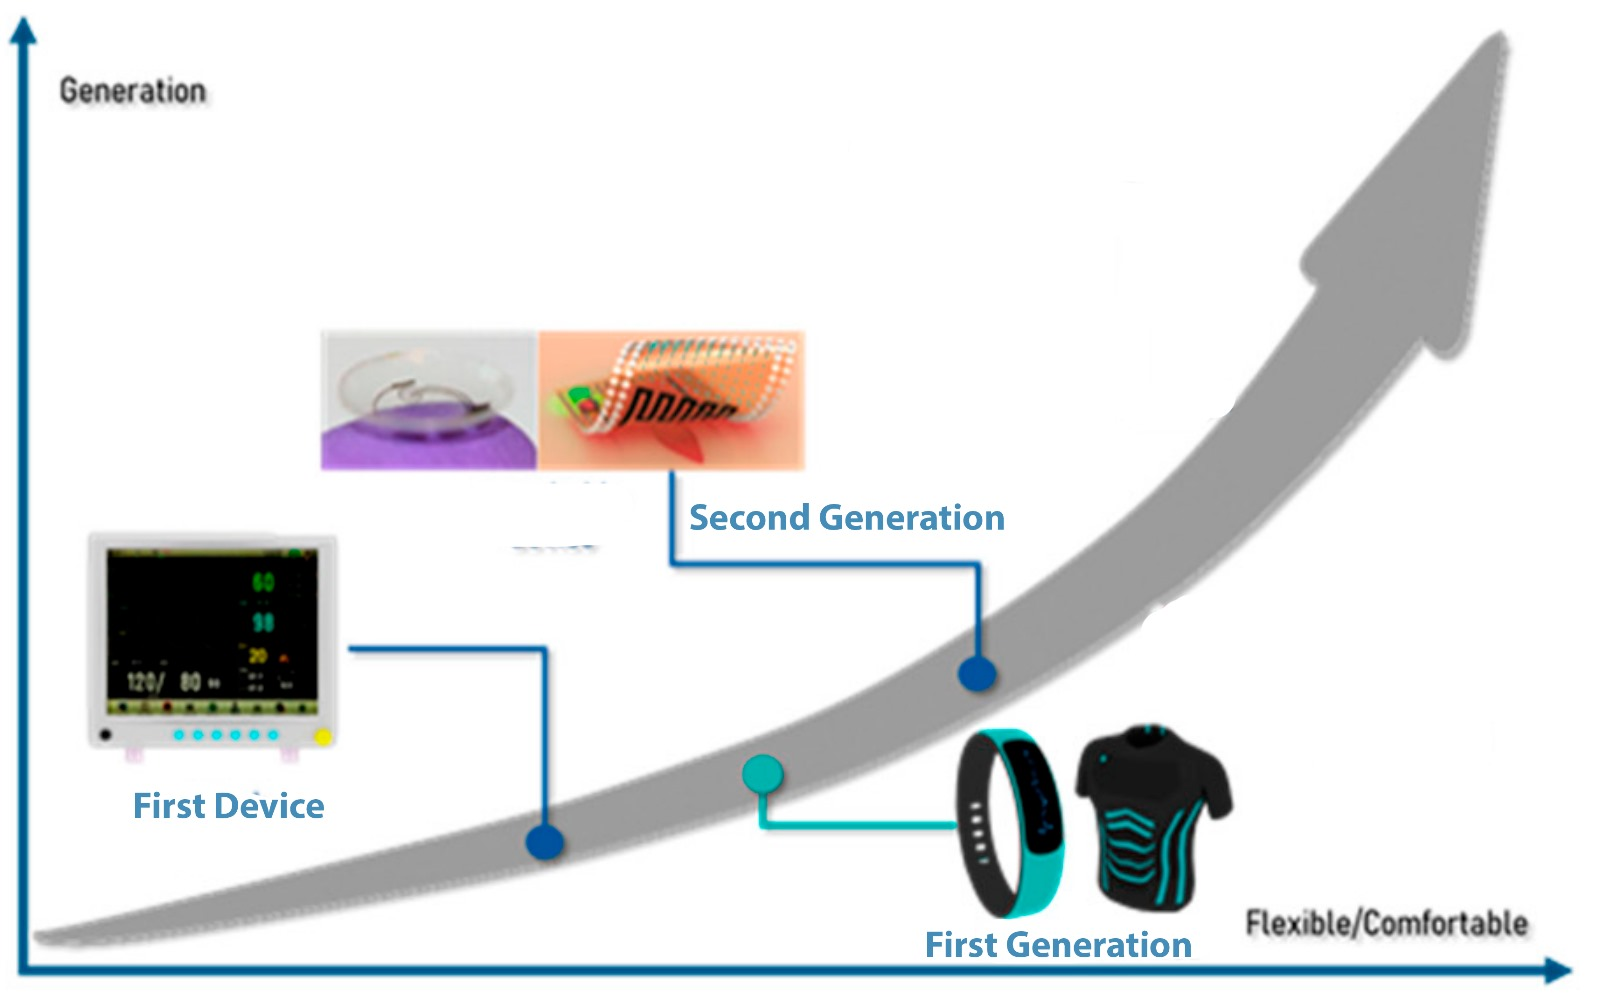
\includegraphics[width=3in]{Wearables_SEB_2024-2025_Group1/Figuras/history.jpeg}
    \caption{Historical evolution of WMDs (adapted from~\cite{Ates2022}).}

    \label{fig:histoy}
    \end{figure}

    \subsection{Impact of Technological Advancements}

    Technological advances in materials sciences, sensor miniaturization, and wireless communication have been instrumental in the evolution of WMDs. The integration of flexible electronics, advanced sensors, and energy harvesting technologies has allowed for more sophisticated and user-friendly wearables. The transition from bulky devices to compact, comfortable and efficient devices has significantly improved user adoption and broadened the scope of wearable medical applications~\cite{Ates2022}.

    The evolution of wearables also reflects a shift from simply monitoring vital signs to providing personalized health insights and even predictive analytics. This transformation has been supported by the development of more advanced data processing capabilities, often leveraging cloud computing and artificial intelligence, to provide meaningful health feedback to users and healthcare providers~\cite{Ates2022}.

\section{Architecture of Wearable Medical Devices}
\label{4.Architecture}
    \subsection{Core Components of Wearable Medical Devices}

    The communication architecture of WMDs involves multiple layers to ensure efficient data flow and secure information sharing. The data flow begins with the sensors collecting physiological signals, which are then processed locally to filter out noise and extract key features. The processed data are then wirelessly transmitted to a smartphone or gateway device, which then forwards the information to a remote server or cloud platform for further analysis and storage (Figure \ref{fig:architecture})~\cite{Saifuzzaman2021,Ates2022}.

    The data collected by wearable devices are often shared with healthcare providers, allowing real-time monitoring and timely intervention when necessary. This architecture facilitates personalized healthcare by providing actionable information to both patients and healthcare professionals, ultimately leading to improved health outcomes~\cite{Guk2019}.

    \begin{figure}[ht]
    \centering
    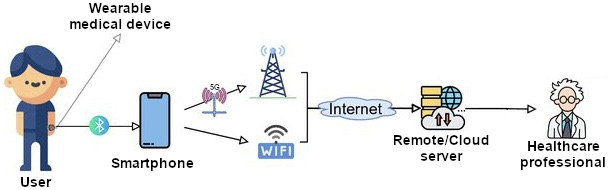
\includegraphics[width=3in]{Figuras/architecture.jpeg}
    \caption{Architecture of a wearable medical device (adapted from~\cite{Saifuzzaman2021}).}
    \label{fig:architecture}
    \end{figure}
    
        \subsubsection{Wearable Sensor Module}
        
        The wearable sensor module is responsible for collecting physiological data such as heart rate, body temperature, or blood glucose levels. These sensors are often integrated into comfortable materials that can be worn on the skin, such as patches or textile fabrics. Sensors are designed to be highly sensitive, energy-efficient and non-intrusive to ensure continuous monitoring without discomfort~\cite{Saifuzzaman2021}.
        
        \subsubsection{Data Transmission Unit}
        
        The data transmission unit handles the communication between the wearable sensor module and external devices, such as smartphones or cloud servers. Typically, data are transmitted wirelessly via technologies such as Bluetooth, Wi-Fi, or near-filed communication (NFC)~\cite{Guk2019}. This wireless connection allows the data collected by the wearable device to be transmitted in real time to a local device or remote healthcare provider for analysis and monitoring~\cite{Nahavandi2022}.

        \subsubsection{Data Processing and Storage System}
        
        The data processing and storage system includes both local and cloud-based components. Initially, raw data are processed by a microcontroller embedded in the wearable device itself to extract useful information, such as calculating the heart rate from an ECG signal. Subsequently, the processed data is transmitted to a smartphone or cloud server for long-term storage, advanced analysis, and sharing with healthcare professionals~\cite{Veeravalli2017}.

    \subsection{Power Supply and Energy Harvesting}
    
    The power supply is a critical aspect of WMDs, as continuous monitoring requires a reliable source of energy. Most wearable devices are powered by rechargeable batteries, but recent advances have explored energy-harvesting techniques to extend battery life or even eliminate the need for charging. Energy can be harvested from various sources, such as body heat, movement, or ambient light, providing a more sustainable power solution for wearable devices~\cite{Ates2022}.


    \subsection{User Interface and Interactivity}
    
    The user interface of WMDs is an important aspect of their architecture, as it determines how easily users can interact with the device. Modern wearable devices feature user-friendly interfaces, often accessible through mobile applications, that display health metrics in an easy-to-understand format. The interface may include alerts and notifications to prompt users to take specific actions, such as adjusting their activity level or seeking medical attention according to the collected data~\cite{Nahavandi2022}.


\section{Applications of Wearable Medical Devices}
\label{5.Applications}

WMDs have a wide range of applications in healthcare, fitness, rehabilitation, and chronic disease management. Their ability to provide real-time data and continuous monitoring has transformed the way medical care is delivered, allowing a more personalized approach to healthcare and empowering patients to play a proactive role in their health management~\cite{Hindelang2024, Babu2024, Cusack2024}.

    \subsection{Health Monitoring and Chronic Disease Management}

    One of the primary applications of WMDs is monitoring health parameters and managing chronic diseases. These devices provide continuous real-time monitoring of vital signs such as heart rate, blood pressure, respiratory rate, and blood glucose levels~\cite{Dias2018}. This continuous monitoring helps patients with chronic diseases such as diabetes, hypertension, or asthma maintain better control over their condition and provides healthcare professionals with valuable data to inform treatment decisions.

    Wearable devices such as the FreeStyle Libre by Abbott have allowed people with diabetes to monitor their glucose levels non-invasively, reducing the need for frequent fingerstick tests~\cite{Ates2022, Luo2024}. Similarly, smartwatches and other wearable health monitors are now capable of detecting irregular heart rhythms, alerting users to seek medical attention before a condition becomes critical~\cite{Cusack2024}.

    \subsection{Sports and Fitness Applications}

    WMDs are widely used in sports and fitness to monitor physiological responses during exercise and recovery. Devices such as fitness trackers and heart rate monitors help athletes optimize their training, track performance metrics, and avoid injury~\cite{Iqbal2016}. Metrics such as heart rate variability, oxygen consumption, and physical activity levels are used to assess fitness progress, identify overtraining, and guide personalized exercise plans~\cite{Cusack2024}.

    For athletes and fitness enthusiasts, wearables provide essential data that enable them to fine-tune their workouts and understand the impact of physical exertion on their bodies. These devices also play an important role in rehabilitation programs by monitoring progress and helping healthcare professionals adjust treatment plans as needed~\cite{Cusack2024}.

    \subsection{Remote Patient Monitoring and Telemedicine}

    WMDs have been pivotal in the growth of remote patient monitoring and telemedicine. By continuously collecting health data and transmitting them to healthcare providers, WMDs facilitate early diagnosis and timely interventions without requiring patients to visit healthcare facilities. This has been particularly beneficial for elderly patients and those in remote or underserved areas~\cite{Dias2018, Nahavandi2022, Babu2024}.

    Remote patient monitoring has also been shown to be valuable in postoperative care, allowing healthcare providers to monitor patients as they recover at home. By providing a direct link between the patient and the healthcare team, wearable devices reduce hospital readmission rates and improve patient outcomes~\cite{Dias2018}.

    \subsection{Rehabilitation and Assistive Technologies}

    WMDs are widely used for rehabilitation purposes, particularly in patients recovering from surgery, stroke, or musculoskeletal injuries. Exoskeletons and other portable devices provide physical support and help regain mobility, allowing patients to exercise effectively in physical therapy~\cite{Dias2018 ,Hemapriya2017, Babu2024}.

    These devices also serve as assistive technologies for people with physical disabilities, improving their independence and quality of life. Examples include smart prosthetics and devices that assist in regaining muscle function, which are designed to adapt to user movements and provide support during daily activities~\cite{Dias2018}.

    \subsection{Mental Health and Wellness}

    WMDs have also found applications in the monitoring of mental health and wellness. Devices that track sleep patterns, stress levels, and physiological indicators related to mental well-being, such as heart rate variability, help users manage stress and improve sleep quality~\cite{Iqbal2016}. With insights into their mental state, users can make lifestyle adjustments or seek medical help to maintain their mental health.

    \subsection{Public Health and Epidemiology}

    WMDs can be used for large-scale data collection, providing valuable information on public health trends. The data collected from the wearables can be anonymized and used to study population health, detect outbreaks, and develop preventive health strategies~\cite{Cusack2024}. For example, during the COVID-19 pandemic, wearable devices were used to monitor symptoms and track the spread of the virus, contributing to public health responses.

    \subsection{Applications in High-Stress Professions}

    WMDs have also been used to monitor the physiological responses of individuals working in high-stress environments, such as first responders, firefighters, and military personnel. By tracking vital signs such as heart rate, body temperature, and hydration levels, wearable devices help ensure the safety and well-being of these professionals and enable early intervention when abnormal physiological responses are detected~\cite{Lu2020}.

\section{Materials Used in Wearable Medical Devices}
\label{6.Materials}

The development of WMDs is highly dependent on the materials used in their construction. These materials must be biocompatible, flexible, durable and capable of accurately interfacing with the human body to collect physiological data. Advances in material science have enabled the creation of wearable devices that are comfortable, functional, and adaptable to various health applications~\cite{Luo2024}.

    \subsection{Key Material Types}

        \subsubsection{Flexible Polymers}

        Polymers such as silicones, polyurethanes, and thermoplastic elastomers are commonly used in WMDs because of their flexibility and comfort. These materials are soft and stretchable and can conform to the body, making them ideal for wearable sensors that need to maintain contact with the skin without causing discomfort~\cite{Trovato2022, Tsikriteas2021}.

        Hydrogels are also utilized for their moisture retention properties, which make them suitable for skin-contact applications. Hydrogels can adapt to dynamic changes in the skin, making them ideal for use in sensors and electrode interfaces~\cite{Trovato2022}.

        \subsubsection{Metal-Based Materials}

        Metals such as gold, silver, and platinum are often used in WMDs for their excellent electrical conductivity and biocompatibility. These materials are typically used in electrodes for ECG and electroencephalography (EEG) sensors, providing reliable electrical interfaces for measuring biopotentials~\cite{Kim2017}.

        Liquid metals, such as gallium-based alloys, are gaining traction because of their ability to retain conductivity while being flexible. This allows for the creation of stretchable circuits that can be integrated into wearables, providing both flexibility and functionality~\cite{Lu2020}.

        \subsubsection{Graphene and Carbon Nanotubes}

        Graphene and carbon nanotubes are materials with unique mechanical, electrical, and thermal properties, making them ideal for wearable applications that require high sensitivity and low power consumption. These carbon-based materials are used in sensors that monitor parameters such as heart rate, respiration, and glucose levels, due to their high conductivity and flexibility~\cite{Kim2017}.

        Their use in biosensors allows for the detection of biochemical markers in bodily fluids, offering a non-invasive way to monitor health.

        \subsubsection{Textile-Based Materials}

        Textiles have become a popular material choice for wearable devices, allowing sensors to be integrated into clothing. Conductive textiles, made by weaving conductive fibers or coating fabrics with conductive materials, enable the seamless integration of sensors into everyday clothing, transforming regular clothing into health monitoring tools~\cite{Song2024}.

        These textile-based devices provide comfort and wearability while allowing continuous monitoring of physiological parameters such as heart rate, muscle activity, and body movement.

        \subsubsection{Ferroelectric Materials}

         Ferroelectric materials are also used for their unique ability to generate electrical charges in response to mechanical deformation, making them ideal for pressure and motion sensors in wearable devices~\cite{Tsikriteas2021}.

        \subsubsection{Phase Change Materials (PCMs)}

        PCMs are used in wearable devices for thermal management. These materials can absorb or release heat during phase transitions, helping to maintain a stable temperature for the wearer. PCMs are particularly useful in wearables designed for personal thermal regulation, ensuring comfort during different environmental conditions~\cite{Yang2024}.

        \subsubsection{Fiber Bragg Grating (FBG)}

        Wearable sensors utilizing FBG technology are widely used in the healthcare sector to monitor physiological metrics and track human movement. Known for their exceptional sensitivity, along with resistance to corrosion and electromagnetic interference, FBG sensors measure precise changes in wavelength induced by variations in temperature, strain, or pressure~\cite{Song2025}. 


    \subsection{Advances and Challenges in Material Science}

    Recent advances in materials science have focused on developing stimuli-responsive materials, such as hydrogels that respond to changes in temperature or pH, to enhance the functionality of wearable devices. However, challenges remain in achieving long-term stability, scalability, and multifunctionality of materials while ensuring cost-effectiveness~\cite{Trovato2022}.

    Another area of development is the integration of energy-harvesting materials to create self-powered wearable devices. The use of piezoelectric materials, which generate electricity from body movements, and thermoelectric materials, which convert body heat into energy, represents a promising direction to make wearables more autonomous and user-friendly~\cite{Pantrangi2024}.

\section{Advantages and Disadvantages of Wearable Medical Devices}
\label{7.Advantages}

WMDs offer numerous advantages, such as real-time monitoring and improved patient engagement, which are transforming healthcare. However, these devices also face several challenges that limit their effectiveness and widespread adoption. Understanding both benefits and drawbacks is essential to advance the development and use of wearable medical technologies~\cite{Dias2018,Iqbal2016,Ha2018}.

    \subsection{Advantages}

        \subsubsection{Continuous Health Monitoring}

        WMDs provide continuous real-time monitoring of vital signs such as heart rate, blood pressure, and glucose levels. This capability allows for the early detection of health anomalies and timely intervention, improving patient outcomes~\cite{Dias2018}.

        Continuous monitoring can be particularly beneficial for the treatment of chronic diseases, such as diabetes or hypertension, as it allows better disease control and personalized healthcare interventions.

        \subsubsection{Remote Healthcare and Telemedicine}

        WMDs enable remote health monitoring, allowing healthcare providers to track patient data without requiring in-person visits. This feature is especially valuable for elderly patients, those with mobility problems, and people living in remote areas~\cite{Nahavandi2022}.

        Remote monitoring reduces the need for frequent hospital visits and helps reduce healthcare costs while maintaining high-quality care.

        \subsubsection{Non-Invasive and User-Friendly}

        Most wearable devices are non-invasive, which makes them comfortable for long-term use and reduces the risk of complications associated with invasive monitoring methods~\cite{Iqbal2016}. Examples include smart watches and adhesive skin patches that measure physiological parameters without the need for needles or catheters.

        Advances in flexible materials and ergonomic design have made these devices comfortable, allowing users to seamlessly integrate them into their daily lives.

        \subsubsection{Improved Patient Engagement}

        Wearables empower users to take an active role in managing their health by providing them with real-time data about their physiological status. This increased awareness encourages healthier lifestyles and promotes adherence to treatment plans~\cite{Iqbal2016}.

        \subsubsection{Data Collection for Public Health}

        Data collected from wearable devices can be aggregated and analyzed to identify public health trends, detect outbreaks, and improve preventive healthcare strategies. These data are invaluable for large-scale epidemiological studies and population health management~\cite{Cusack2024}.

    \subsection{Disadvantages}

        \subsubsection{Data Privacy and Security Concerns}

        WMDs continuously collect and transmit sensitive health data, making them vulnerable to data breaches and cyberattacks. Ensuring data privacy and security is a significant challenge that requires robust encryption and cybersecurity measures~\cite{Iqbal2016}.

        Users may also be concerned about how their data are used, shared, and stored, which can impact their willingness to adopt wearable technologies.

        \subsubsection{Limited Battery Life}

        Most WMDs are based on battery power and frequent recharging can be inconvenient for users. Limited battery life can hinder continuous monitoring, particularly in devices that require significant energy to operate sensors and wireless communication modules~\cite{Ates2022}.

        Although energy harvesting technologies are being explored, they have not yet been widely implemented, and battery limitations remain a significant drawback~\cite{Gao2024}.

        \subsubsection{Data Accuracy and Reliability}

        The accuracy of data collected by wearable devices can be affected by external factors such as movement, skin type, or improper placement of the device. This can lead to inaccurate readings, which can result in misdiagnosis or inappropriate treatment~\cite{Lu2020}.

        Wearable devices must undergo rigorous validation to ensure that their measurements are as reliable as those of conventional medical devices.

        \subsubsection{High Cost and Accessibility}

        The cost of WMDs can be prohibitive for many users, particularly those in low-income regions. Advanced materials, manufacturing processes, and sensors contribute to the high costs of these devices, limiting their accessibility and widespread adoption~\cite{Liu2018}.

        \subsubsection{Material Durability and Comfort}

        Wearable devices are exposed to various environmental conditions, including sweat, movement, and mechanical stress. The materials used must be durable enough to maintain performance over time, and some devices can degrade or become uncomfortable with prolonged use~\cite{Luo2024}.

        \subsubsection{Integration with Healthcare Systems}

        Integrating wearable devices with existing health systems and electronic health records (EHRs) remains a challenge. Compatibility issues, lack of standardization, and the need for interoperability of data limit the seamless flow of information between devices and healthcare providers~\cite{Ravizza2019}.

\section{Regulatory Standards and Requirements}
\label{8.Regulatory}

To ensure the safety, efficacy, and quality of WMD, strict regulatory standards and requirements must be followed, as these regulations are designed to protect users and ensure that devices meet rigorous medical standards. Although different regions have their own regulatory frameworks, they share a focus on core principles such as quality, safety, risk management, and clinical validation. Furthermore, in the pre-market phase, clinical trials must be conducted in accordance with these standards to ensure that the devices meet the necessary safety and performance criteria, identified in Figure~\ref{fig:roadmap}~\cite{Dias2018,Ravizza2019,EuropeanUnion2024}.

\begin{figure}[ht]
\centering
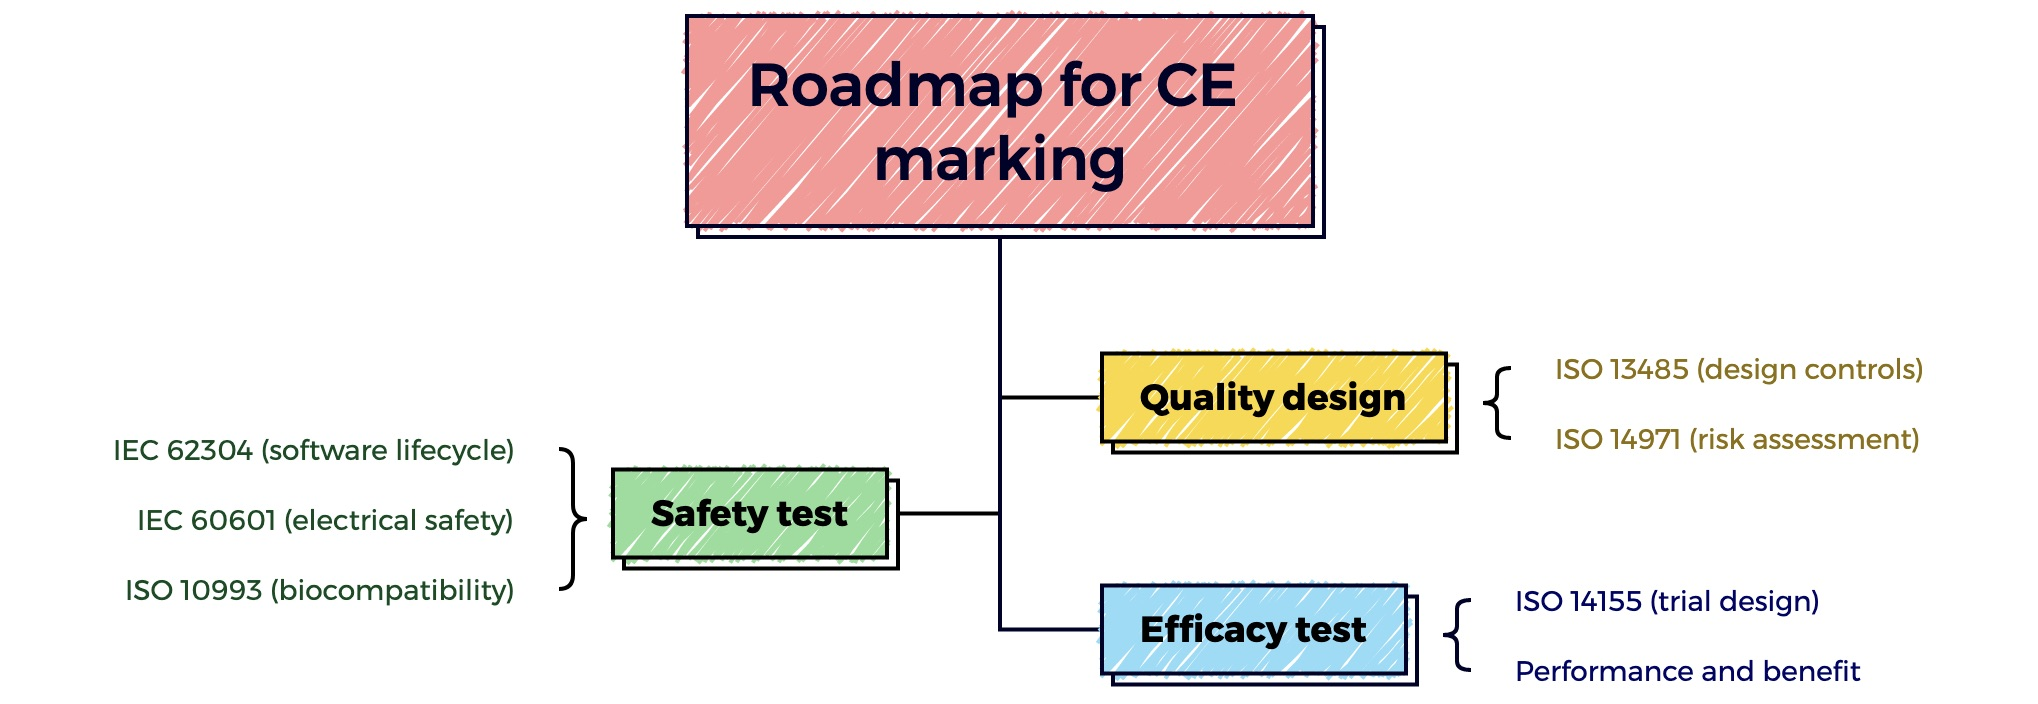
\includegraphics[width=3in]{Figuras/Roadmap for CE marking.jpeg}
\caption{Roadmap for CE marking (adapted based on~\cite{Ravizza2019}).}
\label{fig:roadmap}
\end{figure}

    \subsection{Regulatory Frameworks}


    In the United States, the FDA oversees the regulation of WMDs by classifying devices into three risk-based classes: Class I (low risk), Class II (moderate risk) and Class III (high risk) - where Class I devices are generally exempted from pre-market notification, and Class II and III devices require pre-market clearance (510 (k)) or pre-market approval (PMA), respectively, while also addressing cybersecurity concerns in wearable devices to minimize data breach risks through design and testing standards~\cite{Dias2018,Ravizza2019,FDA2016,FDA2023}. In the European Union, WMDs are regulated under the Medical Device Regulation (MDR 2017/745), which came into effect in May 2021 and similar to the FDA classifies devices based on their risk profile, imposing more stringent requirements for devices of higher risk, and focusing on clinical evaluation and post-market surveillance to ensure continuous monitoring of performance and safety under real-world conditions~\cite{EuropeanUnion2024}.

    Regulatory agencies around the world often align with ISO (International Organization for Standardization) and IEC (International Electrotechnical Commission) to ensure global harmonization of medical device regulations. ISO 13485 provides guidelines for establishing a quality management system (QMS) for medical devices, ensuring consistency in design, manufacturing, and testing~\cite{ISO2016}. ISO 14971 focuses on risk management throughout the device lifecycle, helping manufacturers identify and mitigate potential risks associated with the use of WMDs~\cite{ISO2019}.

        \subsubsection{Biocompatibility and Electrical Safety}

        For WMDs, it is essential that materials are biocompatible, meaning they must avoid causing irritation or adverse skin reactions, as evaluated under ISO 10993 standards~\cite{ISO2018}, while ensuring durability under conditions like sweating, stretching, and prolonged use to maintain performance and comfort~\cite{Chen2020}, and electrical components must comply with IEC 60601 to meet electrical safety, electromagnetic compatibility, and essential performance standards to prevent hazards such as electrical shock~\cite{IEC2012}.
        
        \subsubsection{Software Life Cycle and Cybersecurity}

        Wearable devices that include software components must adhere to \textbf{IEC 62304}, which outlines the lifecycle of software development, including risk management, testing, and maintenance requirements~\cite{IEC2006}.

        Ensuring cybersecurity is crucial for wearable devices, particularly those that collect and transmit sensitive health data. The FDA and MDR require manufacturers to implement cybersecurity measures, such as encryption and secure communication protocols, to protect user data from unauthorized access.

        \subsubsection{Clinical Evaluation and Post-Market Surveillance}

        Both the FDA and MDR require manufacturers to perform clinical evaluations to demonstrate the safety and efficacy of WMDs. These evaluations involve clinical trials and the collection of data on device performance in actual use~\cite{Dias2018}.

        Post-market surveillance involves continuously monitoring the performance of the device after it has been introduced to the market. This includes collecting user feedback, analyzing adverse events, and updating risk assessments as needed~\cite{EuropeanUnion2024}.

    \subsection{Challenges in Regulatory Compliance}

        \subsubsection{Navigating Different Regulatory Requirements}

        One of the key challenges for manufacturers is navigating the different regulatory requirements of various regions. The FDA, MDR, and other regulatory bodies have different processes and documentation requirements, making it difficult for companies to achieve compliance across multiple markets~\cite{Ravizza2019,EuropeanUnion2024,FDA2023}.

        \subsubsection{Cost of Compliance}

        The cost of compliance with regulatory standards can be substantial, particularly for small manufacturers. The need for extensive testing, clinical trials, and documentation adds to the overall cost and time required to bring a wearable medical device to market~\cite{Ravizza2019}.

\section{Challenges and Future Directions}
\label{9.Challenges}

The WMD industry has made significant strides in healthcare, but several challenges must be addressed to fully realize its potential. The future of WMDs will depend on overcoming these challenges, improving device capabilities, and integrating new technologies to expand their application in healthcare~\cite{Lu2020, Babu2024}.

    \subsection{Challenges}

        \subsubsection{Data Privacy and Security}

        Ensuring data privacy and security is one of the most critical challenges for WMDs. These devices collect and transmit sensitive health data, making them vulnerable to cyberattacks and unauthorized access. Manufacturers must implement robust encryption, authentication protocols, and cybersecurity measures to protect user data~\cite{Iqbal2016}.

        Regulatory compliance with data protection laws, such as General Data Protection Regulation (GDPR) in Europe and Health Insurance Portability and Accountability Act (HIPAA) in the United States, is essential to address privacy concerns and build user trust.

        \subsubsection{Battery Life and Energy Efficiency}

        Wearable devices are often limited by their short battery life, which can impact their effectiveness in continuous health monitoring. Although energy harvesting technologies are being explored as a solution, the development of devices with longer-lasting and more efficient power sources remains a major challenge~\cite{Ates2022,Gao2024}.

        \subsubsection{Data Accuracy and Reliability}

        The accuracy of data collected by WMDs can be affected by external factors, such as improper placement, user movement, or skin type. Inaccurate readings can lead to misdiagnosis or inappropriate medical interventions. Manufacturers must focus on improving sensor quality and validation to improve data reliability~\cite{Lu2020, Babu2024}.

        \subsubsection{User Compliance and Comfort}

        For wearable devices to be effective, users must wear them consistently. User compliance can be hindered by discomfort, inconvenience, or the perception of limited benefit. Developing lightweight, ergonomic, and unobtrusive designs that fit seamlessly into daily life is essential to improve user compliance and device adoption~\cite{Luo2024, Hindelang2024}.

        \subsubsection{Integration with Healthcare Systems}

        The smooth integration of wearable devices with healthcare systems, such as EHRs, remains a significant challenge. The lack of standardization and data interoperability issues hinder the efficient use of wearable data in healthcare decision making~\cite{Cusack2024, Ravizza2019}.

        \subsubsection{Regulatory and Compliance Issues}

        WMDs must comply with various regional regulations, such as those set by the FDA and MDR. Navigating these regulatory requirements can be time consuming and costly, particularly for small and emerging manufacturers. Streamlining regulatory pathways and aligning standards between regions could help facilitate broader market entry~\cite{Babu2024,Ravizza2019}.

    \subsection{Future Directions}

        \subsubsection{Artificial Intelligence and Machine Learning Integration}

        The integration of artificial intelligence (AI) and machine learning (ML) can enhance the capabilities of WMDs by enabling real-time data analysis, pattern recognition, and predictive insights. Wearables driven by AI can provide personalized recommendations, detect early signs of health problems, and improve overall health outcomes~\cite{Nahavandi2022, Babu2024}.

        \subsubsection{Advancements in Materials and Energy Harvesting}

        Future wearable devices will benefit from advances in materials science, such as the development of flexible, biocompatible, and stretchable materials that improve comfort and functionality. Energy harvesting technologies, such as piezoelectric and thermoelectric materials, have the potential to create self-powered devices that eliminate the need for regular charging~\cite{Pantrangi2024}.

        \subsubsection{Expanding Applications in Mental Health and Wellness}

        WMDs are increasingly being used to monitor mental health, including stress, anxiety, and sleep patterns. Future wearables will incorporate more sophisticated sensors and algorithms to provide real-time mental health information and support well-being. These devices will play a critical role in promoting mental wellness and facilitating early intervention for mental health problems~\cite{Iqbal2016}.

        \subsubsection{Personalized Healthcare and Precision Medicine}

        WMDs are well positioned to contribute to personalized healthcare by collecting individual health data over extended periods. These data can be used to tailor medical treatments, create personalized health plans, and enable precision medicine. Using AI and continuous monitoring, wearable devices can support proactive healthcare and improve patient outcomes~\cite{Cusack2024}.

        \subsubsection{Integration with Telehealth and Remote Monitoring}

        The COVID-19 pandemic highlighted the importance of remote healthcare solutions. Future wearable devices will increasingly be integrated into telehealth platforms, enabling remote monitoring and virtual consultations. This will improve access to healthcare services for patients in remote or underserved areas and reduce the burden on healthcare facilities~\cite{Nahavandi2022, Cusack2024}.

        \subsubsection{Collaboration and Standardization}

        Greater collaboration between device manufacturers, healthcare providers, and regulatory bodies is essential for the standardization of WMDs. Establishing common standards for data interoperability, cybersecurity, and device validation will facilitate the integration of wearable devices into mainstream healthcare and improve their acceptance~\cite{Ravizza2019}.




\section{Conclusion}
\label{10.Conclusion}

Wearable medical devices (WMDs) hold immense promise in the transformation of healthcare by providing continuous monitoring, enabling personalized care, and facilitating remote health management. These devices enable patients to take an active role in their health, provide healthcare professionals with valuable real-time data, and offer significant benefits, such as early detection of health problems and enhanced patient engagement.

However, for WMDs to fully realize their potential, several challenges must be addressed. The issues related to data privacy, battery life, sensor accuracy, regulatory compliance, and integration with healthcare systems hinder the widespread adoption of these technologies. Overcoming these obstacles will require advances in material science, sensor technology, cybersecurity, and energy efficiency. In addition, collaboration between manufacturers, healthcare providers, and regulatory bodies is crucial to establishing standards that ensure safety, interoperability, and reliability.

The regulatory landscape for wearable medical devices is complex and varies between regions, but the overarching goal is to ensure safety, efficacy, and quality. Adherence to regulatory standards, such as those established by the FDA, MDR, ISO, and IEC, is essential for manufacturers seeking to bring safe and effective devices to market. Harmonizing these standards and addressing regulatory challenges related to standardization and cost will be key to accelerating the adoption of wearable technologies in healthcare care.

In the future, the integration of emerging technologies, such as artificial intelligence, machine learning, and advanced materials, will greatly enhance the capabilities of WMDs, making them smarter, more autonomous, and easier to use. Wearables are expected to expand their role in mental health monitoring, personalized medicine, and telehealth, providing broader applications beyond traditional healthcare settings.

In summary, wearable medical devices represent a transformative shift in healthcare delivery. By addressing current challenges and leveraging technological advancements, WMDs can significantly improve patient outcomes, improve the efficiency of the healthcare system, and empower people to manage their health more effectively. The journey ahead will require not only technological innovation but also a commitment to building an ecosystem that ensures the safe, effective, and equitable use of wearable medical technologies.


% references section

% can use a bibliography generated by BibTeX as a .bbl file
% BibTeX documentation can be easily obtained at:
% http://mirror.ctan.org/biblio/bibtex/contrib/doc/
% The IEEEtran BibTeX style support page is at:
% http://www.michaelshell.org/tex/ieeetran/bibtex/
\bibliographystyle{IEEEtran}
% argument is your BibTeX string definitions and bibliography database(s)
\bibliography{Ref1}
%





% that's all folks
\end{document}


